%!TEX root = article.tex
\begin{figure}[t]
    \centering
    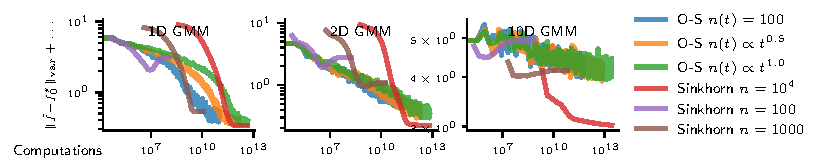
\includegraphics{online_0.01_False_test.pdf}
    \caption{Online Sinkhorn consistently estimate the true regularized OT potentials. Convergence here is measured in term of distance with potentials evaluated on a "test" grid of size $n=10^4$. Online-Sinkhorn can estimate potentials faster than sampling then scaling the cost matrix.}
    \label{fig:potentials}
\end{figure}

\begin{figure}[t]
    \centering
    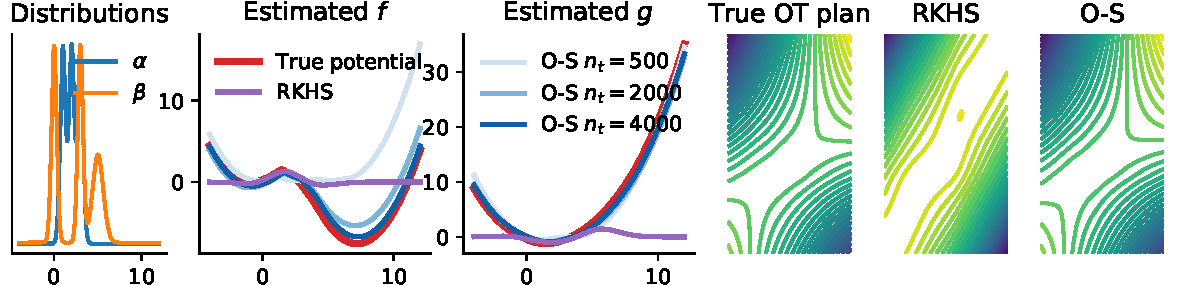
\includegraphics[width=\linewidth]{continuous.pdf}
    \caption{Online Sinhkorn finds the correct potentials over all space, unlike SGD over a RKHS parametrization of the potentials. The plan is therefore correctly estimated.}
    \label{fig:potentials}
\end{figure}

\begin{figure}[t]
    \begin{minipage}{.7\textwidth}
    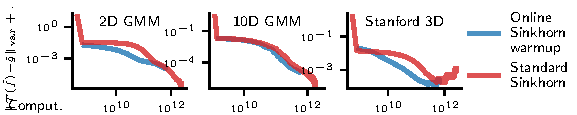
\includegraphics{online+full_0.001_err.pdf}
    \caption{Online Sinkhorn allows to warmup Sinkhorn during the evaluation of the cost matrix, and to speed discrete OT.}
    \label{fig:potentials}
    \end{minipage}%
    \begin{minipage}{.29\textwidth}Test
    \end{minipage}
\end{figure}

\section{Experiments}\label{sec:exps}

% We have introduced and stated convergence results on the online Sinkhorn
% algorithm. These convergence results are non-quantitative and therefore
% require an experimental validation. Our experiments are three-fold: first, we
% show that online Sinkhorn correctly estimates the solutions of \eqref{eq:wass}
% and the Sinkhorn distance, overcoming the bias due to the fixed a priori
% sampling of the regular Sinkhorn algorithm. Then, we show how online Sinkhorn
% accelerates the Sinkhorn algorithm, by progressively estimating sketches of
% the dual potentials, in parallel to the computation of the distance matrix.
% Finally, we show how online Sinkhorn allows one to estimate accurately the
% geometry of the dual, significantly improving the result using SGD with RKHS
% expansions~\citep{2016-genevay-nips}.


The major purpose of online Sinkhorn (O-S) is to handle OT between continuous
distributions.  We first show that it is a valid alternative to applying Sinkhorn on a single realization of continuous distributions, using Gaussian mixture of distributions of various dimension
. We illustrate how O-S accurately estimates the geometry of
the Kantorovich dual in 1 and 2D, significantly improving the result using SGD with RKHS
expansions~\citep{2016-genevay-nips}. Finally, we show that O-S
provides an efficient warmup method to accelerate Sinkhorn on real discrete problems (shapes from Stanford repository).


\subsection{Consistent estimation of continuous OT}\label{sec:exp1}


% We first consider a discrete distribution $(\alpha, \beta)$, to be able to
% compute the reference distance $\Ww = \Ww(\alpha, \beta)$ and the optimal
% potentials $f^\star$, $g^\star$, using Sinkhorn algorithm. The goal here is not
% to perform better than the Sinkhorn algorithm in the long run. Indeed, the
% constraints of online Sinkhorn impose unnecessary slow-downs when dealing with
%  discrete distributions with small supports. Rather, our purpose is to illustrate the improved
% precision of online Sinkhorn for estimating true OT distances. We choose $\alpha$ and $\beta$ to be two
% discrete 1-D distributions, $\Xx=\RR$, sampled from the continuous densities
% displayed in
% \autoref{fig:potentials}. We set $\varepsilon = 10^{-2} \max_{x,y}
% C(x,y)$, where we use the squared Euclidean loss (regularized $\Ww_2$
% setting)---the distributions $\alpha$ and $\beta$ have bounded support. We use
% $\eta_t = \frac{1}{\sqrt{t}}$ for online Sinkhorn and a fixed batch-size $n$, in
% all experiments. We compare the performance of Sinkhorn, online Sinkhorn and
% random Sinkhorn, measuring $\Vert f - f^\star \Vert_{\text{var}} + \Vert g -
% g^\star \Vert_{\text{var}}$ and the absolute error $| \Ww_t - \Ww |$ versus the
% number of computations performed---the evaluation of $C(x_i, y_i)$ and the
% computation of each addition in the $C$-transform being considered as elementary
% computation units. We further report the performance of using out-of-loop
% averaging with $\gamma_t = \frac{1}{\sqrt{t}}$.

\subsection{Continuous potential estimation}

\paragraph{Data and validation.}We measure the performance of our algorithm in a
truly continuous setting, where $\alpha$ and $\beta$ are  parametric
distributions (Gaussian mixtures in 1D and 2D and 10D, with 3, 3 and 5 modes),
from which we draw samples. In the absence of reference potentials $(f^\star,
g^\star)$ (which cannot be computed without a method akin to ours), we compute
"test" potentials $(\tilde f^\star, \tilde g^\star)$ on $\hat \alpha_0$ and
$\hat \beta_0$ of size $N=10000$, using Sinkhorn. We then compare O-S to
Sinkhorn algorithms of various size ($N=100,1000, 10000)$, trained on
realizations independent from the reference grid. To measure convergence, we
compute $\delta_t = \Vert \hat f_t - \tilde f^\star \Vert_{\var} + \Vert \hat f_t - \tilde
f^\star \Vert_{\var}$. This distance is not expected to go to $0$, as we use
test potentials. On the other hand, we expect it to converge with time to a
certain value $\Vert f_\infty - \tilde f^\star \Vert_{\var} + \Vert g_\infty -
\tilde g^\star \Vert_{\var}$. We plot



we monitor the
trajectories of the potentials, and compare them to the discrete potentials for
realization $\hat \alpha$ and $\hat \beta$ of size $N=5000$. We set $n_T = 5000$,
$\epsilon = 10^{-1} \max C$, $\eta_t = \frac{1}{\sqrt{t}}$ and $n(t) = 50 t$.

\paragraph{Comparison to SGD.}\label{sec:compare}
%
We consider a competing approach \citep{2016-genevay-nips}, in which $f_t(\cdot)$
is parametrized as $\sum_{i=1}^{n_t} \alpha_t \kappa(\cdot, x_i)$ (and similarly for
$g_t$), where $\kappa$ is a reproducing kernel (typically a Gaussian). This
differs significantly from online Sinkhorn, where we express $e^{-f_t}$ as a
Gaussian mixture. The dual problem \eqref{eq:sinkhorn} is solved using
stochastic gradient descent, with convergence guarantees on the dual energy.  As
advocated by the authors, we run a grid search over the bandwidth
parameter~$\sigma$ of the Gaussian kernel to select the best performing runs. 

\paragraph{Results.} We show the trajectories of the potentials $(\hat f_t, \hat g_t)$ in
\autoref{fig:potentials}, in 1D. Online Sinkhorn refines the potentials $(f_t, g_t)_t$
until convergence. As we use a parametrization~\eqref{eq:param}
adapted to the dual problem, the algorithm quickly identify the correct shape of
the optimal potentials---as predicted by \autoref{prop:convergence_true}. In
particular, O-S estimates potentials with much less errors than SGD on RKHS in
areas where the mass of $\alpha$ and $\beta$ is low. This allow to consistently estimate the transport plan. The SGD method did not converge
for $\epsilon < 10^{-1} \max C$, while online Sinkhorn remains stable. Online
Sinkhorn does not require to set a bandwidth parameter.



\paragraph{Results.} We report convergence curves in \autoref{fig:convergence}.
Compared to the subsampled Sinkhorn algorithm that computes a biased estimate of
the distance $\Ww$ (purple), the online Sinkhorn algorithm successfully
estimates the distance and the associated potentials, despite performing only
partial $C$-transforms (red). Random Sinkhorn (blue) finds a decent estimation
of the distance and potentials, with fewer computations than the full Sinkhorn
algorithm, but fails to converge. Averaging the random Sinkhorn iterations finds
a biased estimation. The vanilla online Sinkhorn yields values that are much
closer to the true OT distance, albeit with a rather high iterate variance (note
that this variance does reduce---this is a log-log plot). Remarkably, the
out-of-loop averaging of online Sinkhorn enjoys much better converging
property---we confirmed this finding on many synthetic problems. It is
surprising that an averaging mechanism brings speed-up in a non-convex
setting---we attribute this to the convexity of the original problem, although
this should be further investigated.


\subsection{Accelerating the first Sinkhorn iteration}\label{sec:accelerating}

The discrete Sinkhorn algorithm requires to compute the full cost matrix $\hat C \eqdef
(C(x_i,y_i))_{i,j}$  of size $N \times N$, prior to estimating the
potentials $f_1$ and $g_1$ by a first $C$-transform. In contrast, online Sinkhorn can progressively
compute this matrix while computing first sketches of the potentials. We therefore
assess the performance of the following \textit{online+full Sinkhorn} algorithm
in a discrete setting: online Sinkhorn is run with batch-size $n$ during the first iterations, until
observing each sample of $[1,N]$, i.e. until the cost matrix $C$ is completely evaluated. The discrete instantion of online Sinkhorn is derived in \autoref{sec:sinkhorn_discrete}, \autoref{alg:discrete_online}. 
At this point (iteration $t$), online Sinkhorn provides the estimates $f_{t},
g_{t}$. From then, the algorithm only performs full Sinkhorn updates.


\paragraph{Results.} We report convergence curves in
\autoref{fig:early_compute}. The proposed scheme indeed provides an improvement
upon Sinkhorn algorithm. After $N^2$ computations (the cost of estimating the
full matrix $\hat C$), both the function value and distance to optimum are lower
using our scheme: the full Sinkhorn algorithm then operates from a better
initialization of the potentials. Computing those potentials costs approximately as much as
estimating the matrix $\hat C$ in dimension $1$. The \textit{online+full}
Sinkhorn algorithm then maintains an advantage over the full Sinkhorn algorithm
over time. Note that the cost of estimating initial potentials becomes negligible
as the dimension increases---the cost of computing $\hat C$ dominates. This
strongly advocates for using an online scheme as a warm-up for regularized OT
estimation. We note that using smaller batch-size $n$ may lead to higher speed-up (here, $n=50$ performs better than $n=100$), so that in practice, there is an optimal $n$. The speed gain decreases with $\epsilon$, but remains
significant even for $\epsilon = 10^{-4} \max \hat C$. We also noted that
using a sampling-without-replacement scheme brings an additional speed-up. Out-of-loop averaging is also beneficial. We refer to \autoref{sec:supp_exp} for an additional experiment with a smaller $\varepsilon$.
